\tikz \draw (0,0) node{1} (1,0) node{4} (2,0) node{3} (3,0) node{2} (4,0) node{5};

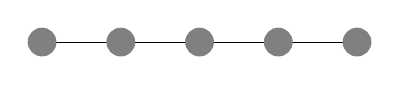
\begin{tikzpicture}

\draw (0,0) -- (4,0);
\filldraw [gray] (0,0) circle (5pt) [gray] (1,0) circle (5pt) [gray] (2,0) circle (5pt) [gray] (3,0) circle (5pt) [gray] (4,0) circle (5pt);
\end{tikzpicture}

\tikz \draw (0,0) node{1} (1,0) node{2} (2,0) node{3} (3,0) node{4} (4,0) node{5};


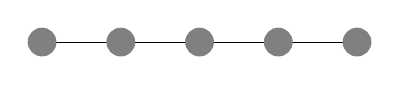
\begin{tikzpicture}

\draw (0,0) -- (4,0);
\filldraw [gray] (0,0) circle (5pt) [gray] (1,0) circle (5pt) [gray] (2,0) circle (5pt) [gray] (3,0) circle (5pt) [gray] (4,0) circle (5pt);


\end{tikzpicture}